\scanpage{34}
\mspage{1}
Systèmes spéciaux de cinq points sur une sphère complexe (plus gén.\textsuperscript{t} sur une \deleted{\unsure{courbe}} droite projective sur un corps alg clos \(k\) \unsure{de car. \(0\)})

Ce sont les systèmes \((\Sigma,K)\) avec \(K\subset\Sigma\), \(\operatorname{card}K=5\), et tels qu’il existe un autom. non trivial de \((\Sigma,K)\) --- i.e. le groupe \inserted{\(G\)} des automorphismes de \((\Sigma,K)\) n’est pas réduit à \(1\). On fait la classification suivant la structure de ce groupe.

Soit \(g\in G\) d’ordre maximal. On peut identifier \(g\) à une permutation de \(I\), et la discussion se fait suivant la structure de celle-ci. Notons que \deleted{l’ordre de \(g\ne1\) est} tout autom. d’ordre fini de \(\Sigma\) \deleted{\(\unsure{\nu}\,g\) d’ordre \(5\)} a exactement deux pts fixes, et que \deleted{\unsure{il est}} \inserted{si l’ordre est \(\nu\)}, \(\mathbb Z/\nu\mathbb Z\) opère librement sur \(\Sigma\setminus\Sigma^g\). Cela montre que
\[
K=K^g\amalg\text{orbites d’ordre }\nu,\quad\text{donc }2\leq\nu\leq5.
\]
\margin{l’opération est celle de \(\mu_\nu\) sur \(\widehat{\mathbb G}_m\)}

\textcircled{1} \(\nu=5\), alors \(K\) est une orbite --- OPS que c’est l’orbite \(\mu_5(k)\) de \(\mu_5\) opérant sur \(\mathbb P^1_k\). Le groupe total des autom. est \tikz[baseline=(d.base)]{\node[draw,circle,inner sep=1pt] (d) {\(\mathbb D_5\)};}. À isom. près, il y a un seul tel cas.

\margin{Structure pentagonale sur \(I\) (``pentagone'')}
\figure{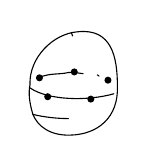
\begin{tikzpicture}[scale=.75,line cap=round,line join=round]
\draw (-.73,-.03) .. controls (-.75,.43) and (-.34,.84) .. (.08,.87)
 .. controls (.65,.93) and (.75,.45) .. (.75,-.05)
 .. controls (.77,-.58) and (.42,-.87) .. (-.05,-.88)
 .. controls (-.39,-.89) and (-.60,-.73) .. (-.68,-.53)
 .. controls (-.74,-.34) and (-.76,-.16) .. (-.73,-.03);
\draw (-.73,-.08) .. controls (-.43,-.29) and (.23,-.31) .. (.69,-.18);
\draw (-.60,.09) .. controls (-.36,.18) and (-.25,.14) .. (-.08,.18)
 .. controls (.01,.19) and (.09,.17) .. (.17,.16);
\draw (.41,.14)--(.44,.12);
\draw (.59,.07)--(.61,.02);
\foreach \x/\y in {-.57/.09,.02/.19,.59/.05,-.43/-.23,.30/-.27}
 {\fill (\x,\y) circle(1.7pt);}
\draw (-.68,-.53) .. controls (-.47,-.58) and (-.25,-.60) .. (-.08,-.60);
\draw (-.03,.86)--(-.01,.80);
\end{tikzpicture}}

\textcircled{2} \(\nu=4\) alors \deleted{\(\unsure{K|\Sigma}=\operatorname{card}I^g=1\)} \inserted{\(K^g=\{P\}\)}, et \(I\setminus\{P\}\) est une orbite. OPS que c’est \(\mu_4\), sur lequel \(\mu_4\) opère, et \(P\) est un pôle : \(\unsure{\infty}\). Le groupe total des autom. est \(\mathbb Z/4\mathbb Z\simeq\mu_4(k)\).

La catégorie de ces configurations est équivalente à celle des carrés orientés.

\margin{``pyramide carrée''}
\figure{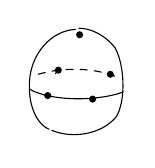
\begin{tikzpicture}[scale=.75,line cap=round,line join=round]
\draw (-.02,.89) .. controls (-.43,.87) and (-.78,.48) .. (-.80,-.01)
 .. controls (-.82,-.49) and (-.62,-.74) .. (-.47,-.80);
\draw (-.42,-.82) .. controls (-.05,-.97) and (.43,-.88) .. (.67,-.59)
 .. controls (.84,-.31) and (.81,.29) .. (.65,.58)
 .. controls (.45,.83) and (.20,.91) .. (.04,.91);
\draw (-.80,-.12) .. controls (-.44,-.33) and (.35,-.33) .. (.79,-.17);
\draw[dash pattern=on 2.6pt off 2.5pt] (-.65,.13)
 .. controls (-.25,.25) and (.30,.25) .. (.69,.08);
\foreach \x/\y in {.05/.80,-.49/-.23,.27/-.29,-.31/.20,.57/.13}
 {\fill (\x,\y) circle(1.7pt);}
\draw (-.31,.20)--(-.36,.14);
\end{tikzpicture}}

\textcircled{3} \(\nu=3\), Alors \deleted{\(\unsure{\Sigma|K}\)} \(\operatorname{card}K^g=2\), \inserted{donc \(K^g=\Sigma^g\)}, et \(I\setminus K^g\) \inserted{\(=J\)} est une orbite,
\deleted{Le groupe total est}
\inserted{qu’on peut supposer \(\mu_3\).} La catégorie de ces configurations est équivalente : celle des triangles combinatoires i.e. celle \(\mathrm{Ens}(3)\) des ens \(J\) de card \(3\).

A \(J\) on associe \(\Sigma_J\deleted{\unsure{\Sigma}}\) avec \(J\cup P_J\) (\(P_J\subset\Sigma_J^{\unsure{g}}\) ens des deux pôles de \(\Sigma_J\) pour corr. \(1\)-\(1\) avec l’ens \(\omega(I)\) des or. de \(J\), si \(\unsure{k|K}=\mathbb C\)). Groupe des autom. est \(\mathbb D_3\).

\margin{\unsure{Partition} \(2\) et \(3\) (par ordre de \unsure{cardinaux|valeurs} ou symétries)}
\margin{``bitétraèdre''}
\figure{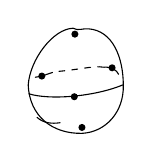
\begin{tikzpicture}[scale=.75,line cap=round,line join=round]
\draw (-.80,-.08) .. controls (-.77,.35) and (-.38,.87) .. (-.04,.88)
 .. controls (.04,.83) and (.13,.88) .. (.22,.87)
 .. controls (.63,.84) and (.81,.39) .. (.81,-.09)
 .. controls (.82,-.53) and (.52,-.88) .. (.11,-.90)
 .. controls (-.39,-.91) and (-.78,-.61) .. (-.80,-.08);
\draw (-.79,-.23) .. controls (-.44,-.34) and (.32,-.28) .. (.80,-.08);
\draw (-.68,.05) .. controls (-.56,.06) and (-.47,.11) .. (-.39,.13);
\draw[dash pattern=on 2.1pt off 2.6pt] (-.28,.15)
 .. controls (.06,.18) and (.33,.25) .. (.47,.22);
\draw (.48,.22) .. controls (.61,.23) and (.70,.17) .. (.73,.10);
\foreach \x/\y in {-.01/.78,.11/-.80,-.02/-.28,-.57/.07,.62/.21}
 {\fill (\x,\y) circle(1.7pt);}
\draw (-.65,-.63) .. controls (-.54,-.73) and (-.40,-.74) .. (-.26,-.72);
\end{tikzpicture}}
\margin{33}
